\section{国際SKAのサイエンス}\label{pulsar.s2}

この節では国際SKAパルサーチームで議論されているサイエンスについてその概要を紹介する。


\subsection{SKAを用いたパルサー探査}
前節で述べたように、パルサーはそれ自身の性質や進化の研究だけでなく、重力波検出、一般相対性理論の検証や銀河系構造の研究などにも利用することができる。これらを推進するためにはSKAを用いてできるだけ多くの新しいパルサーを発見し、そのパルスの特性を詳細に観測しなければならない。そこで必要になるのは、複数のアンテナを用いた高感度探査と、SKA-LowとSKA-Midを相補的に連携させた探査である。

\subsubsection{複数のアンテナを用いた高感度探査}
観測感度を向上させるには、複数のアンテナをコヒーレントに合成する (アンテナからの出力を位相差なく足し合わせる) ことが必要になり、最小検出フラックス$S_\text{min}$はアンテナの個数$N$に反比例する: $S_\text{min}\propto 1/N$。
感度は観測時間によって補えると思われるかもしれないが、データ処理するために必要な時間は観測時間の3乗に比例するため、アンテナを増やすことによって一瞬一瞬の感度を向上させることが重要である。
パルサーのパルス特性は、パルスの周期や dispersion measure (DM) などによって特徴づけられるが、新しいパルサーの場合それらのパラメータの値は未知である。
したがって新しいパルサーを発見するためには、コンピュータによってそれらの値を変えつつ何度もデータ解析しなければならない。
その試行回数は膨大であり、データ解析に用いるコンピュータにはおよそ peta-flops\footnote{FLoating-point Operations Per Second (FLOPS) とは、コンピュータが1秒間に行える浮動小数点数演算の回数であり、コンピュータの計算速度を表す指標である。パルサー探査に必要な 1 peta-flops という計算速度は、1秒間に$10^{15}$回の小数演算を意味する。ちなみに2014年現在、日本のスーパーコンピュータ「京」の計算速度は10 peta-flops、「TSUBAME 2.5」は2 peta-flops、「地球シミュレータ ES2」は0.1 peta-flops である。} の計算速度が必要となる。
さらには、Giant Radio Pulses (GRPs) やRotating RAdio Transients (RRATs; \cite{McLaughlin06}) のようなパルス強度が激変するようなパルス観測に対しては、観測時間をいくら稼いでも無意味であり、アンテナを複数使用することによる瞬時的な感度が不可欠である。

\subsubsection{SKA-Low と SKA-Mid の連携}
SKA-Low と SKA-Mid では観測周波数が異なり、それらを連携させてパルサー探査することが重要である。
宇宙からの電波パルスは星間プラズマによって周波数分散され、地球への到達時刻$t$は周波数$f$を用いて$t \propto \text{DM}\cdot f^{-2}$と表せる。
よって周波数$f$の電波と$f+\varDelta f$の電波の到達時間間隔を$\varDelta t$とすると、$\text{DM} \propto f^{3} \varDelta t/\varDelta f$となり、観測周波数が高いほど大きいDMを観測できると考えることができる。
このことは、観測周波数の低いSKA-Low ではDMの小さいパルサー、つまり地球近傍かあるいは高銀緯のパルサーを探査しやすく、SKA-Midでは低銀緯の遠いパルサーを探査しやすいことを示している。
また電波パルスのスペクトル特性によってもSKA-Low と Mid で観測できるパルサーが異なるため、その二つを相補的に連携させて使用することが重要である。
それによって、図~\ref{pulsar.keane.fig1}に示すSKA Phase~1 では約10,000個のノーマルパルサーと1,800個のミリ秒パルサーの発見が見込まれ、Phase~2 においてはさらにその3倍近い数を発見できるだろう。
\begin{figure}
	\centering
	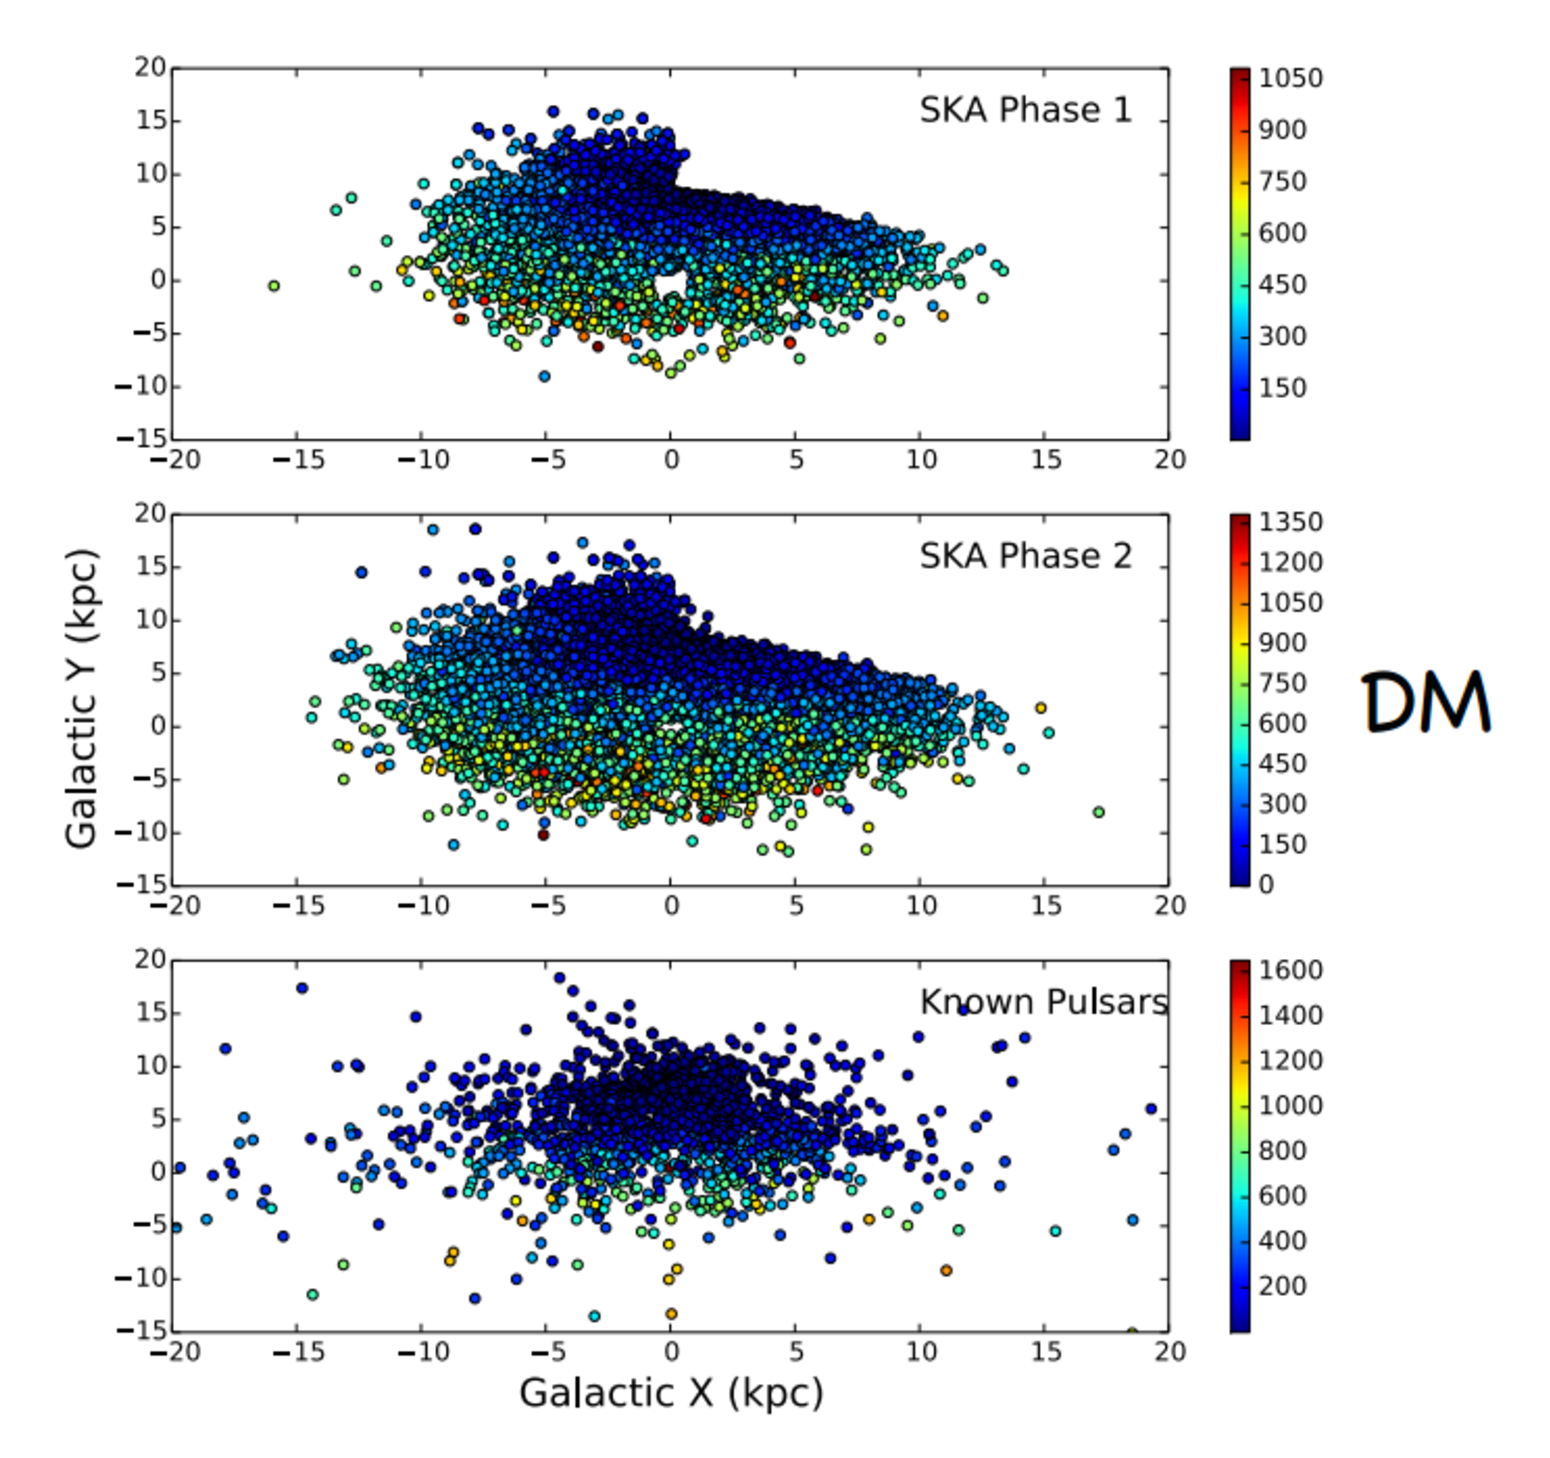
\includegraphics[width=10cm]{pulsar/pulsar.keane.fig1.eps}
	\label{pulsar.keane.fig1}
	\caption{SKA Phase~1, 2 で発見されるであろうパルサーの分布。}
\end{figure}

\subsubsection{まとめ}
パルサー探査では、複数のアンテナを用いた高感度観測とSKA-Low と Mid の連携が重要である。
それによって従来を大幅に超える数の新しいパルサーが発見できるだろう。
また発見されたパルサーのパルスタイミングを正確に取得するためには、追観測を数週間から数か月にわたって何度も行う必要があり、また他の周波数帯で観測するなど条件を変えて観測することも重要である。
そのように新しいパルサーの探査と追観測を行うことによって、中性子星の磁気圏の物理や状態方程式の解明、一般相対性理論の検証などの多くの科学が実現することだろう。


\subsection{天の川銀河中心のパルサー}

天の川銀河の中心には質量が約太陽の400万倍の巨大ブラックホールがあると考えられる。この周囲にパルサーが見つかれば、ブラックホールの近傍の空間を通過するパルサーのパルス信号の変化を精密に調べる事によって、ブラックホールとパルサーを使った強い重力場における一般相対性理論の検証が可能になる。

パルサーは、極めて精確な時計として使用でき、パルサータイミング観測の精度は100マイクロ秒にも至る。これは、天の川銀河中心で数10kmの位置精度に相当する位置変化を検出できる事になる。従って、パルサータイミング観測を行う事によって、ブラックホールの質量とスピンの計測を精密に行える。質量については、百万分の一の精度(1太陽質量の精度に相当)で測定できよう。また、ブラックホールのスピンについては、無次元のパラメーターを求める事によって、ブラックホールの周囲に特異点が発生しないとする宇宙検閲官仮説についての検証を行える可能性がある。更には、ブラックホールの四重極モーメントの測定によって、ブラックホールは質量、スピン、電荷のみで記述できるとする無毛定理の検証も行える可能性がある。

一方、上記の測定結果によって、天の川中心の環境を調べる上で重要な貢献ができる。まず、パルサーを用いたブラックホール質量はブラックホールの距離によらずに決定できるので、10マイクロ秒角の精度を出せる位置天文学観測結果と組み合わせると、ブラックホールが存在する天の川銀河中心までの距離R0(現在約8.3kpcと推定)を1pcより良い精度で決定できるはずである。更に、ブラックホールのスピン量が測定できる事により、現在、実際に撮像を試みているブラックホールの影の形を説明できよう。一方、天の川銀河中心にある個々のパルサーを気象観測局の様に使用して、天の川銀河中心の自由電子、磁場、スキャッタリングの極限状態の環境の測定ができる。

天の川銀河中心のパルサーは、本当に存在するのであろうか。これまでの状況証拠から天の川中心には中性子星が存在する多くの証拠がある。現在でも星生成が続いている事、パルサーの元になるウォルフレイエ星や大質量星の存在、中心の数pc内に厚い星でできた円盤や若い大質量星が存在する事、X線連星システムがチャンドラ衛星により予想より多く存在している事が見つかった事などである。実際、フェルミ衛星により、天の川銀河中心付近にはパルサー状点源が少なくとも見つかっている。また、パルサー風星雲が存在する事や、GeVガンマー線放射を説明する為には、中心の星団にミリ秒パルサーが多数ある必要がある。多波長の観測により、中心1pc以内に1000個程度のパルサーがあるという推定がされている。

以上の間接的な証拠により多数のパルサーが天の川銀河中心に存在すると考えられるが、実際に見つける事は簡単ではない。その理由は、天の川銀河中心は、電波のスキャッタリングが大きいからである。これまで、多くのパルサーサーチが行われてきている。スキャッタリングのため、より高い周波数での観測が必要である。これまで、天の川銀河中心付近の0.5度(距離8.3kpcを仮定すると約70pcに相当)の領域をエッフェルグベルグ100m電波望遠用により10.55GHzでサーベイが行われ、これまで6つのパルサーまたはマグネターが見つかっている。特に、マグネターPSR1745 -2900は、SgrA*と3秒角(0.1pcに相当)のズレしかなく、天の川銀河中心に近い可能性がある。しかし、これでも、ブラックホールの物理量を測定するには十分な近さではない。今後、より周波数が高いパルサーの探査を行い、見つかれば、それを使って研究が進むであろう。


\subsection{SKAによる重力波天文学}
 SKAのパルサータイミングによる重力波検出のメインターゲットは巨大ブラックホール連星からの重力波である。パルサータイミングの周波数帯($10^{-8}$から$10^{-9}$Hz)で観測できるブラックホール連星の質量は典型的に太陽質量の$10^8$から$10^9$倍と非常に重く、銀河中心にあるような連星であると考えられる。また、この周波数帯の重力波を放つ連星は数ヶ月から数年で一周するような軌道を持ち、合体まで長い時間がかかるため、我々が観測するのは軌道周期がほとんど変化しない連星からの単一の周波数の重力波である。このような連星は宇宙に数多く存在するため、様々な方向からやってきた重力波は重なり合って背景重力波を形成する。銀河の分布には偏りがあることから、この背景重力波は非等方成分を持つと考えられる。

 近年、パルサータイミングのデータ解析を工夫してこの重力波の非等方成分を取り出す方法が精力的に研究されている。SKA1-MIDの場合、数十度もしくは数度程度の角分解能で強い重力波が来る方向を特定することができる。さらにSKA2ならば数分角まで分解能を上げることができるため、電磁波対応天体を見つけることで波源の母銀河を特定することが可能になると期待される。波源の位置の特定ができると低赤方偏移のブラックホール連星の分布を知ることができると共に、高赤方偏移の連星で形成される背景重力波の等方成分を取り出すことができる。背景重力波の強度はブラックホールがどのように成長し、合体してきたかに大きく依るため、これによって銀河形成史に制限をつけることが可能になる。

\begin{figure}[t]
\centering
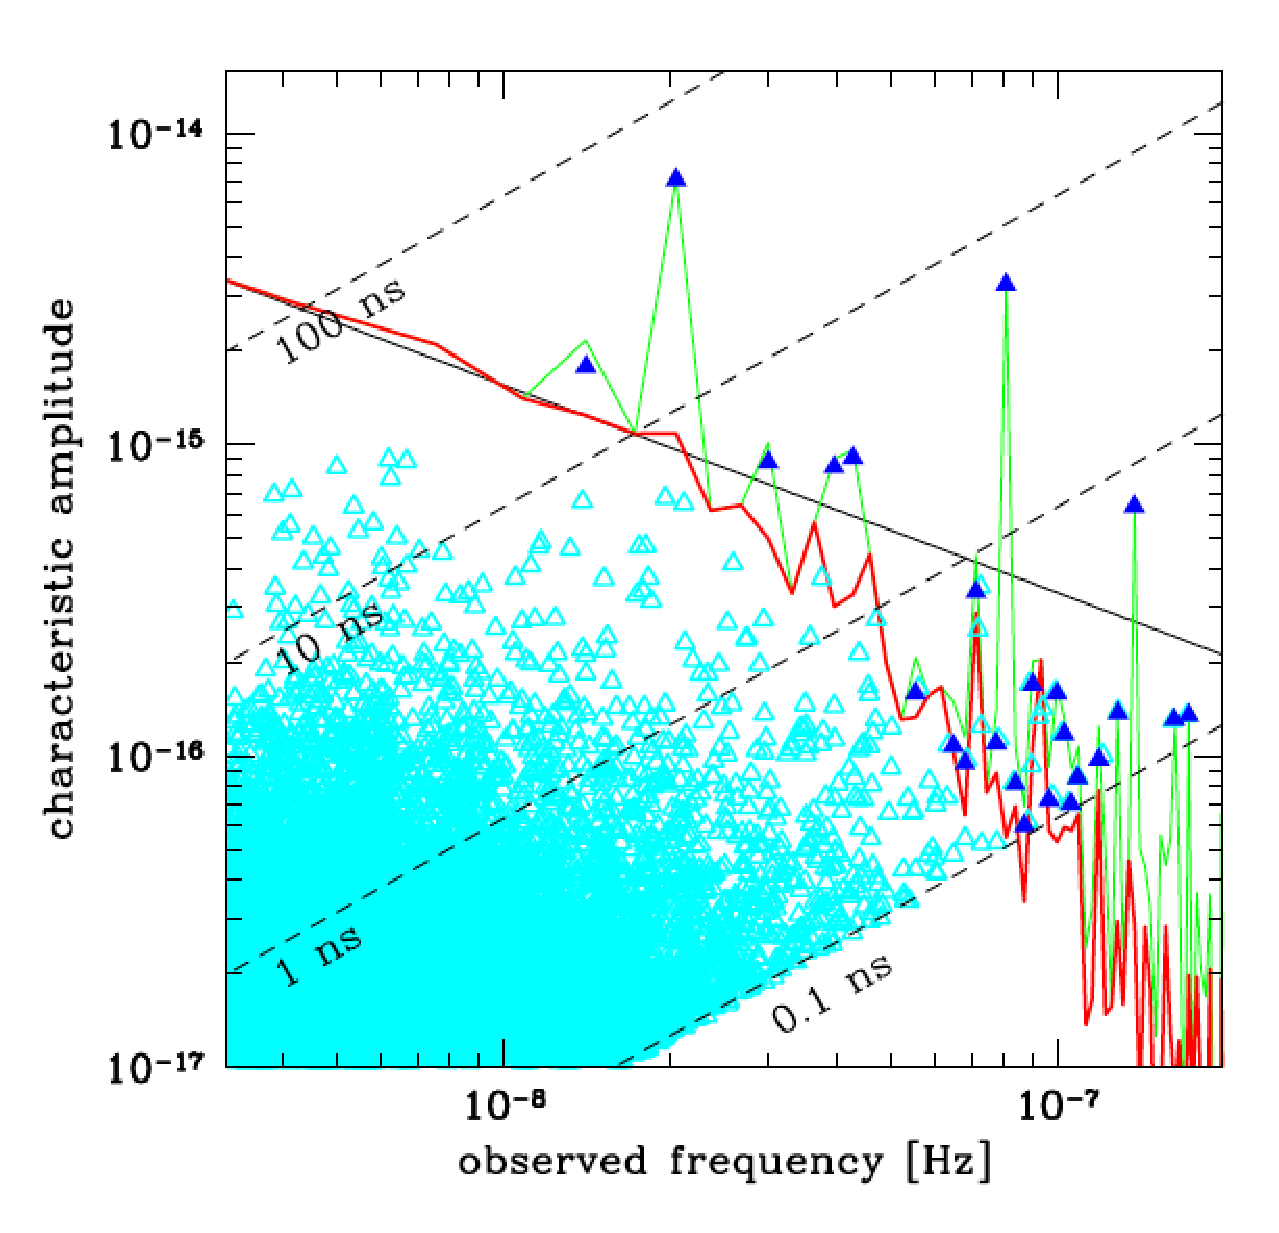
\includegraphics[width=0.6\textwidth]{pulsar/FIG_GW_SMBH.eps}
\caption{シミュレーションにより生成された巨大ブラックホール連星からの重力波\cite{Sesana2013}。縦軸は重力波の強度、横軸は周波数。点線はノイズの大きさを変えたときのパルサータイミングの感度を表す。水色の点は個々の連星からの重力波を表し、緑色の線がすべて足し合わされた背景重力波のスペクトル。青色の点は波源の特定ができる可能性のある連星で赤線はそれらを取り除いたときの背景重力波のスペクトル。}
\end{figure}

 この角度分解能の大幅な向上を可能にするのは年周視差を使った精密な地球とパルサー間の距離測定である。重力波によるパルス間隔の変化は通常、地球の位置が変化による”earth term”とパルサーの位置変化による”pulsar term”の足し合わせの形で書かれ、分離することができない。”pulsar term”は個々のパルサーによって異なる一方、”earth term”は観測するパルサーに依らず同じであることから、通常のデータ解析では複数のパルサー間の相関を取ることで”earth term”だけを取り出す作業を行う。SKA2で可能になる地球とパルサー間の精密な距離測定は、データ解析上ノイズとして寄与する”pulsar term”の情報として使うことができ、これが角度分解能の向上につながる。

 さらに”earth term”と”pulsar term”の分離によって、重力波の時間変化を測ることも可能になる。パルサータイミングに使われるパルサーは1000光年を超える距離のものもあり、遠く離れた地球とパルサーは異なる時刻に重力波源から放出された重力波の影響を受ける。つまり、異なる時刻の重力波の情報を持つ”earth term”と”pulsar term”を独立に測ることで、重力波の時間進化を1000年のオーダーで知ることが可能になる。こうして通常のパルサータイミングの10年オーダーの観測では測れない重力波の周波数の時間変化を調べることで、ブラックホール連星の質量を正確に決めることができるだけでなく、ブラックホールのスピンを測ることも可能になる。

 また、パルサータイミングによる重力波の検出は一般相対論の検証にも役立つ。一般相対論では重力波の偏光モードは2つ($+$と$\times$モード)であるが、重力理論が変更されると偏光は最大で6($+$と$\times$に加えてスカラーモードが2つ、ベクトルモードが2つ)まで増えることが知られている。偏光モードの数は重力理論の修正のされ方によって決まる。異なる偏光モードの重力波は空間の歪め方が異なり、全方向のパルサーのパルス間隔の変化を比べたときに重力波による歪みの空間的なパターンが異なる。そのため、データ解析においてスカラーモードやベクトルモードの歪みのパターンが存在するか検証することで、重力理論の検証が可能である。また、重力波の速度が異なる場合も歪みのパターンが変更を受けるため、同様の方法で重力子が質量を持つ理論を検証することも可能である。

 最後に、パルサータイミング実験は初期宇宙理論の検証にも役立つ。中でも大きな振幅の重力波を予言するのが、宇宙相転移や超弦理論から予言される1次元の位相欠陥「宇宙ひも」である。宇宙ひもは非常に重く相対論的な速度で運動するため、強い重力波を放出する。高赤方偏移において宇宙ひもから放出された重力波は背景重力波を形成し、我々の近くで放出されたものは重力波バーストとして観測される。背景重力波の強度やバーストの頻度分布は宇宙ひもの線密度や数分布に依存し、そこから初期宇宙の理論の情報につなげることができる。例えば重力波の強度を決める線密度は宇宙ひも生成時の宇宙のエネルギースケールに対応するため、パルサータイミングから重力波に制限がつくことで宇宙ひもを予言する理論のエネルギースケールに制限を与えることができる。また、宇宙ひもの他にも振幅の大きい背景重力波を予言する初期宇宙理論は様々なものが存在する。そういった理論の検証にとって重力波強度に強い制限を与えることができるパルサータイミング実験は重要である。

 なお、これら宇宙論起源の背景重力波は巨大ブラックホール連星からの重力波とはスペクトルの周波数依存性が異なる。よって背景重力波の起源を特定するには周波数依存性を精度よく測ることが必要になる。そのためには高い感度での重力波検出が必要であるが、SKAの感度ならば巨大ブラックホール連星起源の背景重力波の周波数依存性を十分な精度で測り、起源の特定が可能であると理論的に見積もられている。




\subsection{Tests of Gravity with Pulsars (パルサーによる重力理論の検証)}

パルサーは、極めて正確に一定の周期でパルス波を放出することが知られているが、
実際に我々が観測するパルス波の到着時刻は一定ではない。
もっとも単純には、観測者である我々に対してパルサーが運動していると、
パルサーが静止している場合と比べてその到着時刻には差異が生じてくる。
パルサーの到着時刻を前後させる要因としては様々なものが考えられるが、 大別して \vspace{3pt} \\
\qquad (1) ~ パルサーのニュートン力学的な運動に起因するもの \vspace{3pt} \\
\qquad (2) ~ パルサーと我々の間に介在する星間物質による影響など、宇宙物理学的起源を持つもの \vspace{3pt} \\
\qquad (3) ~ 一般相対論的な重力による効果 
\vspace{3pt} \\
などが考えられる。
実際に観測されるパルス波の到着時刻のずれから (1) や (2) の効果をさっ引くことができれば、
(3) の重力の効果に起因するずれのみが残り、
それを用いてパルスが放出された場所などの時空の情報を抜き出すことができる。
パルサーを用いた重力理論の検証は、それら抜き出された時空の情報をもとに、
重力理論の検証を行おうというものである。

パルス波の到着時刻を予想する公式は、
「Time of Arrival 公式」、通称「TOA 公式」と呼ばれている。
以下ではこの公式について、
特に (1) と (3) に起因する効果に注目して詳しく述べていく。
(2) に起因する影響は独立に扱うことができるので、以下では特に触れない。 

パルサーが BH のまわりを公転しているとしよう。
BHのまわりのパルサーの運動は第0近似、両者の重心系に対するケプラー運動でよく記述されると期待される。
ケプラー運動は軌道周期や離心率など、5つのパラメータ (以下 K パラメータ)を用いて特徴づけられる。
しかしながら、実際の運動は厳密なケプラー運動で記述されるわけではなく、
それらからのずれを考慮する必要がある。
例えば重力波の放出により系からエネルギーが抜き取られると、公転周期が小さくなることが期待される。
そこで、それらケプラー運動からのずれを特徴づけ、パルサーの運動を
複数のパラメータを用いて定式化したのが、
Parametrized-Post-Keplerian (PPK) フォーマリズムと呼ばれるものである。
特に、軌道周期の変化率など、ケプラー運動からのずれを特徴づける12のパラメータを、
Post-Keplerian (PK) パラメータと呼ぶ。
PPKフォーマリズムにおいてパルサーの運動は、5個の K パラメータと12個の PK パラメータ、合わせて17個のパラメータを用いて完全に記述されることになる。
つまり、パルス波の到着時刻をこれら17個のパラメータの関数として与えることができ、
その公式が TOA 公式である。

ここで重要なことは、PPKフォーマリズムはケプラー運動からのずれを、
背景にある重力理論を仮定することなく一般的に特徴づけている点である。
つまり、TOA 公式は完全に現象論的に作られた公式であり、
そこに現れるパラメータは、観測されるパルス周期のみで原理的には完全に決定され得る。
一方で、ひとたび重力理論を指定してやると、
その重力理論に基づいて PK パラメータを求めるための方程式が得られる。
5つの K パラメータ(${\bm P}_{\rm K}$)とパルサー質量($m_{\rm pul}$)、
BHの質量($m_{\rm BH}$)がわかれば、
その方程式を解くことによって、
PK パラメータの値を理論的に予想する事もできる。
つまり、式で書くと
\begin{equation}
P_{\rm PK}^i=f_{\rm theory} \, ({\bm P}_{\rm K}, m_{\rm pul}, m_{\rm BH}) \,, \qquad
 (i = 1\,, 2\,,  \cdots\,, 12)
\label{eq1}
\end{equation}
という具合だ。
ここで、$P_{\rm PK}^i$は$i$番目のPKパラメータを表す。
この理論的予測と観測結果を比べることによって、
重力理論の検証が可能となる。

それではここで、具体的にどのように重力理論の検証が行われるか、一つの例を紹介しておこう。
簡単のために、Kパラメータがパルス波の観測とTOA公式から精密に決定されているとする。
上で説明したように、
ある重力理論を仮定すると、観測によって決められた K パラメータ (${\bm P}_{\rm K,obs}$) と
パルサー・BHの質量 ($m_{\rm pul}$, $m_{\rm BH}$) を用いて、
全ての PK パラメータの値を理論的に予測することができる。
これは逆に、
1つの PK パラメータ $P^1_{\rm PK}$ を TOA 公式と観測とを比べることによって読み取ることができれば、
\eqref{eq1}式に従って $m_{\rm pul}$ と $m_{\rm BH}$ の間に1つの関係式が与えられることを意味する。
各々の PK パラメータは TOA 公式において独立に寄与するので、
別の PK パラメータを考えることにより、もう1つ独立な関係式を導くことが可能になる。
%
つまり、観測結果から読み取ることのできるPKパラメータの数だけ、
観測精度の範囲内で$m_{\rm pul}$と$m_{\rm BH}$の間に独立な関係を付けることができるのである。
両者の質量を座標軸とするダイアグラムに、
これらの関係を表す曲線を描いたのが図\ref{fig_mass}である。
\begin{figure}[t]
\begin{center}
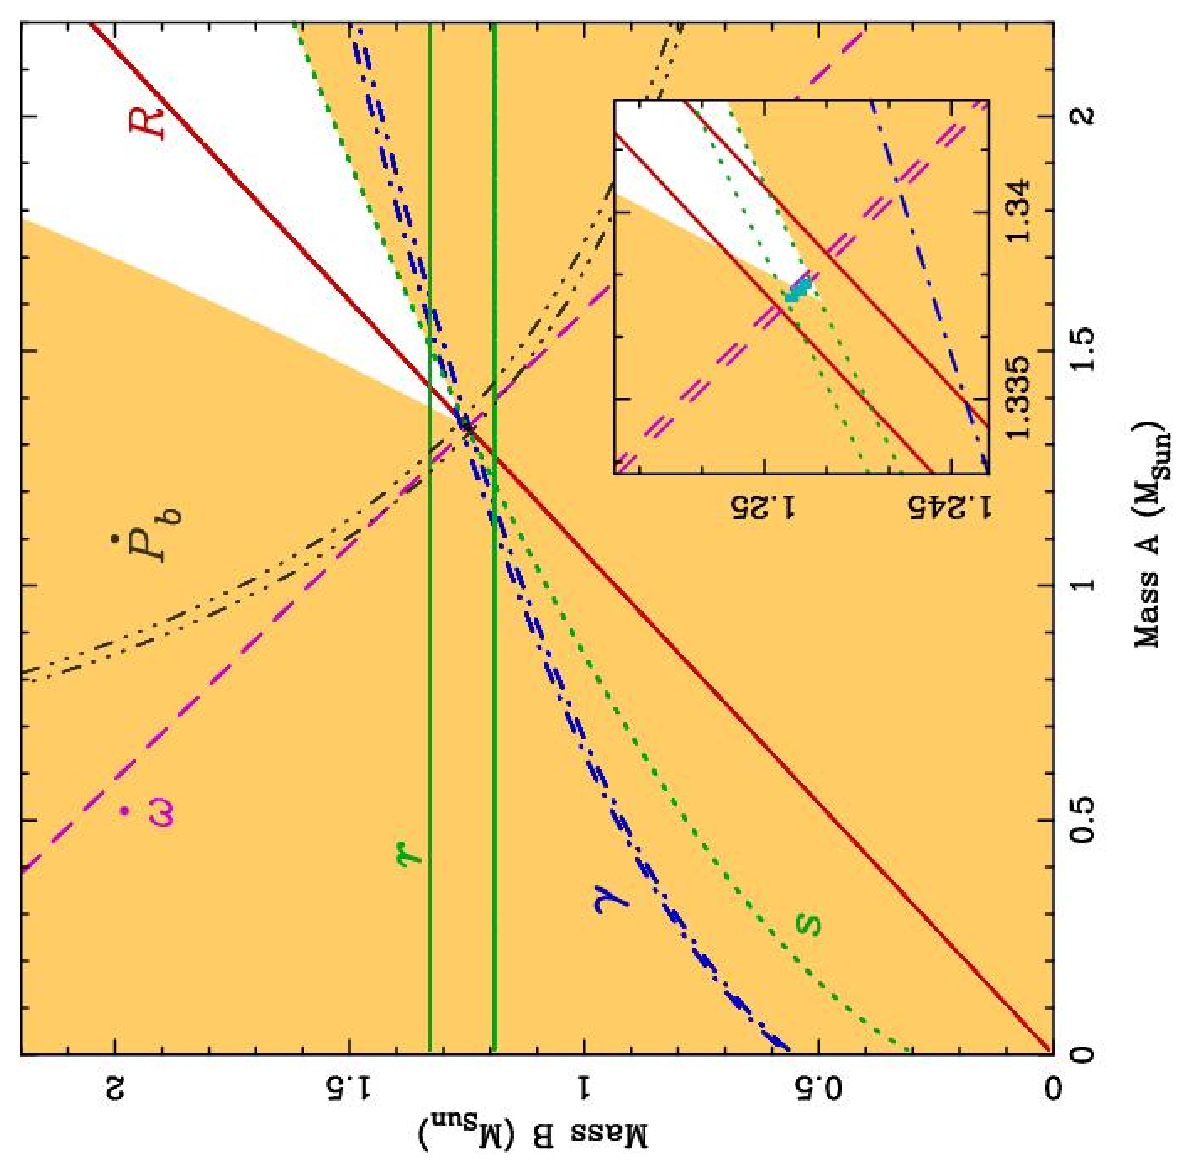
\includegraphics[width=100mm,angle=270]{pulsar/fig_Kramer.ps}
\end{center}
\caption{
ケプラーと Post-Keplerian パラメータを用いて描かれる連星の質量ダイアグラム\citep{Kramer:2006nb}。
}
\label{fig_mass}
\end{figure}
この図において、全ての曲線が一点で交われば、
それは質量を決めるのに用いた重力理論が正しい理論であることを意味する。
一方、新たな別の交点がうまれれば、
それは質量の算出に用いた重力理論が正しくないことを示唆し、
その重力理論を棄却することができる。

上で述べたように、PPKフォーマリズムを用いた
重力理論の検証法は極めて汎用性の高い方法であり、
連星系の運動とパルス波の伝播とを予言可能な重力理論であれば、
どのような理論も検証が可能である。
SKAで観測される連星系パルサーを用いて、このような重力理論の検証を行うことが、
国際SKAが目指しているサイエンスの一つである。



\subsection{パルサー磁気圏}
\subsubsection{Introduction}
SKAを用いることで3万個ものパルサーが見つかり、これまで感度不足のために分からなかった多くの情報を得ることが出来るようになる。パルサー磁気圏の観測ではパルサーの幾何学形状を解析を行い、それにより放出される重力波の大きさを推定することも出来るようになると期待される。

重力波の検出はSKAの主なターゲットの一つである。だが、現在パルサーを用いた重力波の観測に用いることの出来るパルサーの数は極めて少ない。まずは銀河全体に散らばる観測可能なパルサーの数を増やして、電波パルサー、X線パルサーやマグネターに分類し、銀河内のパルサーの三次元的分布図を描き出すこと、さらに、パルサー毎に放射の特徴も異なるためパルサーそれぞれの3D beam構造を観測することが必要である。

50MHzからガンマ線の全ての波長における高感度観測によってパルサー磁気圏のマッピングを行ったり、最新のまたたきをイメージングする技術を駆使するとパルサー磁気圏の将来までも推定することが出来る。

観測によって得られるパルサーからの信号の強度や偏光は必ずパルサー磁気圏を伝搬しその影響を受ける。このことからパルサーの放射過程や幾何学形状を推定し、さらには回転軸の方向を決定し固有運動の方向との一致具合によって超新星爆発時のキックの様子を理解したりパルサー自身の特性と超新星残骸の形状、組成などの関連や生まれた時の自転速度や磁場の決まり方を議論することも出来る。

\subsubsection{Pulsar life}
超新星爆発の残骸として残った中性子星(約 2 $M_{\odot}$)が回転し強い磁場(約$10^{13}G$)を持つ時パルサーとしての活動性を示すようになる(1.1参照)。中性子星の質量と半径の関係は状態方程式に大きな制限を与えているためこれらの観測は非常に重要になっている。

若いパルサーは周期$P$が約$< 0.1$s程度で回転しており、誕生時の双極磁場強度と周期は典型的にはそれぞれ$\sim 10^{12}$G、$10$msecと思われるがその分布についてはよくわかっていない。双極磁場強度がほぼ一定で$P \dot{P}=$一定で徐々にスピンダウンし、パルサーの典型的な年齢は$\tau = P/2\dot{P}$で推定できる。スピンダウン光度が大きく(若く)、近いパルサーはガンマ線で観測されやすい傾向にある。回転が遅くなるとパルスが観測できずdeath line(死線)と呼ばれる領域に達する。

連星系に誕生したパルサーがやがてパルサーとしての寿命を迎えたあとも主星からの質量降着により再び回転エネルギーを得てspin up し、数msという速い周期で回転するミリ秒パルサーへとなる。このときまた高い$\dot{E}$を持ち、
$\gamma$線で放射が観測されている。

これらの詳細な理解に依って銀河系内の中性子星がどのような磁場強度でどのような周期で誕生し、それがどれくらいの頻度であり、超新星爆発の性質とどう関係しているかを知ることで、銀河進化の中での中性子星の役割が理解されることが望まれる。

\subsubsection{geometry}
パルサーの幾何学的構造やビーム形状は高時間分解能、高感度の観測によって決定することが出来る。実際、PSR B0906-49の幾何学的構造は図\ref{fig:pulsar-beam}に示すように高時間分解能の精密な観測によって推定されている\citep{Kramer08}。また、1.4GHz と3.1GHz,8.6GHzでの偏光観測も行われていて、どのような放射が行われているか、またパルサー自身からどの程度の距離で放射が行われているか推定することで放射のメカニズムを決定することが出来る。

\begin{figure}[t]
\begin{center}
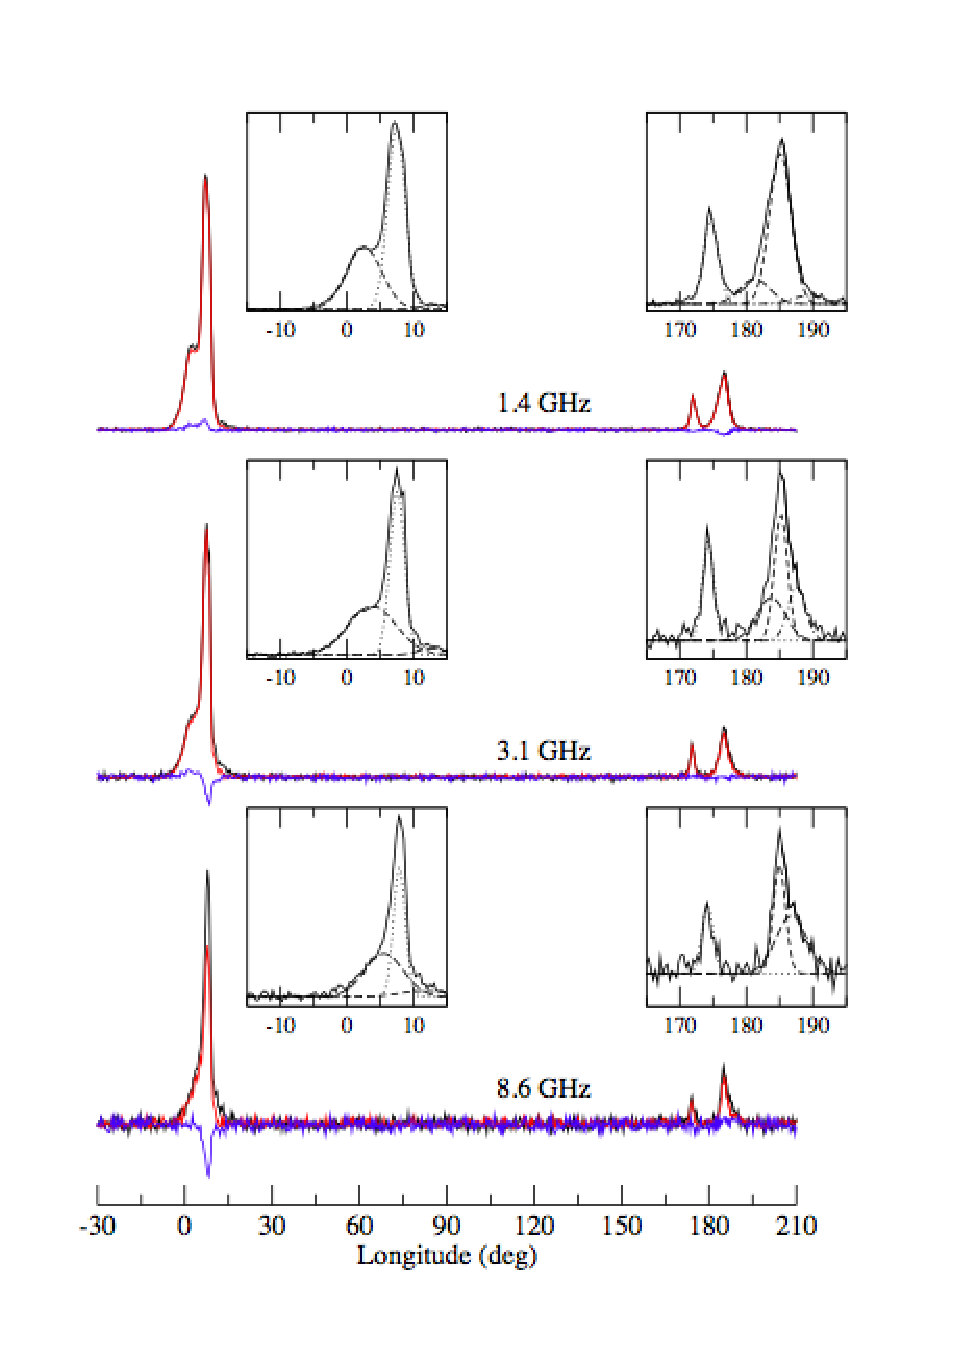
\includegraphics[width=80mm]{pulsar/kumamoto.eps}
\end{center}
\vspace{-1cm}
\caption{PSR B0906−49の直線偏波(赤)と円偏波(青)のプロファイル\citep{Kramer08}。}
\label{fig:pulsar-beam}
\end{figure}

\subsubsection{3D beam}
3D beamの構造の磁気圏伝搬による変化を取り除くことで放射メカニズムの基礎的な特徴を理解することができ、3D beamからの放射のスペクトルをみることでスペクトルインデックス$\alpha$や標準偏差$\sigma$の値を特定しpopulation synthesis modelの正確な構築に寄与出来る。\cite{Bates13}はPSR B1823-13の観測を行い、スペクトルインデックス$\alpha$=-1.41、標準偏差$\sigma$=0.96と値を定めている。さらに、歳差運動などの非対称性によっても幾何学構造や3D beamに制限を与えることが出来る。

パルサー同士の連星では、一方のパルサーの放射が他方のパルサーの磁気圏を通り抜けることを利用して、磁気圏のプラズマの構造を直接探査することが可能になる。実際に、PSR J0737-3039A/B系ではプラズマ密度が非常に高く、パルサー周りのプラズマ領域はパルサーの磁気圧等から推定される半径よりも2倍小さくなることが推定された\citep{Breton12}。SKAによってより多くのパルサー同士の連星が発見されることでパルサー磁気圏のトモグラフィーをすることができ、よりパルサーの構造に迫れることも期待されている。

\subsubsection{millisecond pulsar}
ミリ秒パルサーの放射ビームの構造やパルス間の現象についての理解はまだまだ出来ていない。正確なタイミング観測が必要である。最近の研究でミリ秒パルサーの個々のパルス放射はタイミング観測の安定性に制限を与えることが分かっている\citep{Oslowski14}。一般に、個々のパルスの研究は電波放射機構の特定にとって非常に大切である。

\subsubsection{磁気圏の状態遷移}
パルサーの中にはさまざまタイムスケールでパルス放射を行ったりやめたりするパルサーがある。電波放射のオン/オフやモード変化とスピンダウン率(つまりは、磁気圏電流)の変化が相関していることがわかりつつある。この変化のきっかけは未だ良く分かっていないが磁気圏にいくつかの準安定状態があり状態間の遷移が起こっていると考えられている。放射のオン/オフのスイッチのきっかけやパルス周期の変動(timing residuals)の観測(これによって磁気圏電流変化が分かる)にはSKAによる2週間に1回48時間のパルサーセッションの長い期間のモニタリングが必要である。これらのデータと日本の得意なX線観測と同時観測に依って比較することでパルサー磁気圏現象の理解が一段と深まると予想される。



\subsection{Structure and the Magnetoionic Interstellar Medium}

パルサー電波を用いると,パルサー自身はもとより,星間物質(ISM)に関して,
特に,1)熱的自由電子の分布やその乱流的性質,2)磁場構造について調べることができる.
Keane et al.(2014, ``A Cosmic Census of Radio Pulsars'')によると,
SKAでは$\sim 10000$個程度のパルサーが観測されると算出されている.
現在観測されている$\sim 1000$個に比べて飛躍的に増加するパルサーの電波を用いることで
星間物質の構造がより詳細に明らかになると期待される.

1)電子分布モデルの精密化について

銀河系内自由電子の空間分布モデルとしてNE2001がある
\cite{NE2001}.
これは,電波に加え可視光,X線の観測を元に作られた詳細な電子密度の空間分布である.

電波が伝播してくる空間の平均電子密度を反映した観測量が,
電子密度の視線に沿った積分量DM(Dispersion Measure)である,
$\textrm{DM} = \int_0^d n_e dl$[cm$^{-3}$pc],
ここで,$d$はパルサーまでの距離(pc),
$n_e$は電子密度(cm$^{-3}$)
である.
これは,
パルス到達時刻の周波数による違いから得られる.
SKAによって,
距離が独立に決定されるパルサーが増えると,
太陽$-$パルサー間の平均電子密度がわかり,
銀河系電子密度分布モデルをより精密にすることができる.
これにより,
距離が不明のパルサーについて,
DMからより精度の高い距離の制限を得ることができる.

2)星間ガスの乱流構造について

伝播空間の電子密度揺らぎにより
電波は散乱されシンチレーション等が生ずる.

Thin-screen model(例えばLyne \& Smith, 1990, ``Pulsar Astronomy'')によると,
距離$D$にあるパルサーからの電波がうけるrms散乱角は,
$\theta_{scat} \sim (1/2\pi) \sqrt{D/a} r_e \Delta n_e \lambda^2$,
ここで,$a$は散乱体の典型的スケール,
$r_e$は古典電子半径,$\Delta n_e$は電子密度の揺らぎ,
$\lambda$は電波の波長である.
これは,長波長の電波ほど$\theta_{scat}$が大きいことを示している.

パルサーの電波パルスでは,
pulse broadeningという現象が観測されている.
これは,低周波でのパルスほどパルスの時間幅が長くなる現象であり,
長波長の電波パルスには大きく散乱されている成分が含まれることで解釈できる.
パルスの時間幅を表すpulse broadening time $\tau$は,
screen modelでは,
$\tau \sim D \theta_{scat}^2/(4c) \propto \nu^{-4}$
と表される.
より詳しく,
コルモゴロフ・スケーリング則に従う電子密度揺らぎを考えると,$\tau \propto \nu^{-4.4}$
となり,
これとconsistentな観測が報告されている\cite{LMGKA2004}.

また,$\tau$のDM依存性も観測されている.
コルモゴロフ・スケーリング則に従う密度揺らぎの場合,
$\tau \propto DM^{2.2}$となる\cite{RNB1986}.
一方,これからずれた観測報告もあり,
電子密度揺らぎがコルモゴロフ・スケーリング則に従わない例かもしれない\cite{BHAT2004}.
この様なPulse broadeningの詳細な観測が多く行われると,
電子密度揺らぎの乱流的性質について詳しく議論できるようになる.

Dynamical Spectrumは,
パルス電波強度を時間$-$周波数($t-\nu$)面で見たものである.
これを解析することで,
散乱体である密度揺らぎのサイズや速度について知ることができる.
さらに,($\nu$, $t$)をフーリエ変換した($f_\nu$, $f_t$)面で表した
2ndary spectrumは散乱体の位置について制限することができる
\cite{ST2006}.
2ndary spectrumは,
$f_\nu = a f_t^2$の特徴的な構造を示す.
係数$a$は,$a=(s/(1-s))(\lambda^2 D)/(2 c \mu^2)$で表される,
ここで,$\mu$はパルサーの固有運動を表し,
$s=$(パルサーから散乱体までの距離)/(観測者から散乱体までの距離)である.
したがって,観測される2ndary spetrumから$a$を得ることで,
散乱体の位置を知ることができる.
高精度な時間分解・周波数分解の観測をすることで,
散乱体である電子密度揺らぎの空間分布が決まると考えられる.

DMの時間変動も観測されており,
これは,視線上に分布する電子密度の揺らぎが動くことによる.
変動量としては,
$dDM/dt \sim 10^{-5} - 10^{-3}$ [cm$^{-3}$ pc/yr]
が得られており,
これから,乱流のパワースペクトルや乱流の散逸スケールを予測することができる
\cite{YOU2007}.


3)銀河系の磁場構造について

円盤銀河が大局的磁場構造と乱流磁場を持つことが知られている.
銀河系についても,
系外電波源やパルサーのファラデー回転量RMを用いて,
磁場構造の解析が行われてきた.
ファラデー回転量RMは,
$ \textrm{RM} = 0.81 \int_0^d n_e B_\parallel dl$[rad/m$^2$],
ここで,$d$はパルサーまでの距離(pc),
$n_e$は電子密度(cm$^{-3}$),
$B_\parallel$は磁場ベクトルの視線方向成分($\mu$G)である.
系外電波源のRMには電波源固有の磁場,銀河間空間の磁場からの寄与が含まれるが,
パルサーの場合それらはない.
また,DMも同時に用いることで,
星間磁場の視線成分を評価することができる,
$\langle B_\parallel \rangle = 1.232 RM/DM$ [$\mu$G].

大局磁場の円盤面に平行な成分について,
太陽近傍では,
銀河座標の銀経が約70-90度($l \sim 70^\circ$ - $90^\circ$)の方向へ太陽から離れる方向に
磁場ベクトルが向いているとする結果が1970年代から得られている.
大局磁場の強度は,$\sim 2 \mu$G程度と評価されている.
また,
太陽より銀河中心側と外側で磁場方向が反転する可能性を観測は示している
(例えば,\cite{HAN2006}).

RMは空間的に大きな変動を示す.
これは,乱流磁場やHII領域等からの寄与と考えられる.
この変動が大局磁場の決定を難しいものにしている.
天球上で近接するパルサーのペアをとり,
それらのRMの差$\Delta RM$とDMの差$\Delta DM$を用いることで
パルサーとパルサーに挟まれる空間の磁場強度を得ることできる,
$\langle B_\parallel \rangle = 1.232 \Delta RM/\Delta DM$ [$\mu$G].
この方法を用いると,太陽近傍のHII領域等からの寄与は除くことができる.
SKAによって,
パルサー数が飛躍的に増え,また,高精度でRMが決定されることにより,
より詳細な銀河系磁場構造の決定が可能になる.

銀河系の磁場を正確に知ることは,
銀河間空間の磁場を知るためにも重要である.
銀河間空間の磁場は,系外電波源のRMを用いて評価することができるが,
これには銀河系の寄与が前景成分として含まれる.
銀河系の磁場構造を正確に知ることで,
系外電波源のRMから前景成分を適切に取り除き,
銀河間空間の磁場を正しく評価できる.
また,SKAによって系外銀河中のパルサーが数多く観測されるようになると,
そのRMとDMから銀河間空間の磁場や電子密度分布について評価できるようになり,
宇宙磁場についての理解が一層進むと考えられる.



